% ARM entry for the filtermodule
\chapter{Filter Module} \label{chapter:filtermodule}
The filter module is a reusable entity that holds two sets of filters: the input filters and the output filters. These filters can use objects and conditions, which are also defined in the filter module. 
A filter module is superimposed on a class and the filter module can extend the signature and the behavior of the class on which it is superimposed.

\section*{Syntax}
\begin{lstlisting}[caption = {Filter module syntax}, label = lst::ARM:fm:syntax,
style = listing, language = ebnf, float = tpb]
FilterModule ::= `filtermodule' FilterModuleName [FilterModuleParameters] `{'
                  [Internals] [Externals] [Conditions]
                  [InputFilters] [OutputFilters] `}';
\end{lstlisting}
A filter module has a unique identifier in a concern; the uniqueness is defined over the name and not the name
in combination with the parameters.
The  ordering of the blocks
of a filter module
is fixed, thus it is only possible to use them in the ordering as shown in the syntax of \autoref{lst::ARM:fm:syntax}. The filter module template is demonstrated in
the concern template in \autoref{lst::arm::fm:tmtemplate}.
All the blocks are optional, making it possible to write a completely empty filter module.
\begin{lstlisting}[language={Composestar},style=floatlisting, caption={Filter module template},label={lst::arm::fm:tmtemplate}, floatplacement=tbp]
filtermodule ( ... ) {
  internals
    ...
  externals
    ...
  conditions
    ...
  inputfilters
    ...
  outputfilters
    ...
}
\end{lstlisting}

\section*{Semantics}
\begin{figure}[tpb]
	\centering
	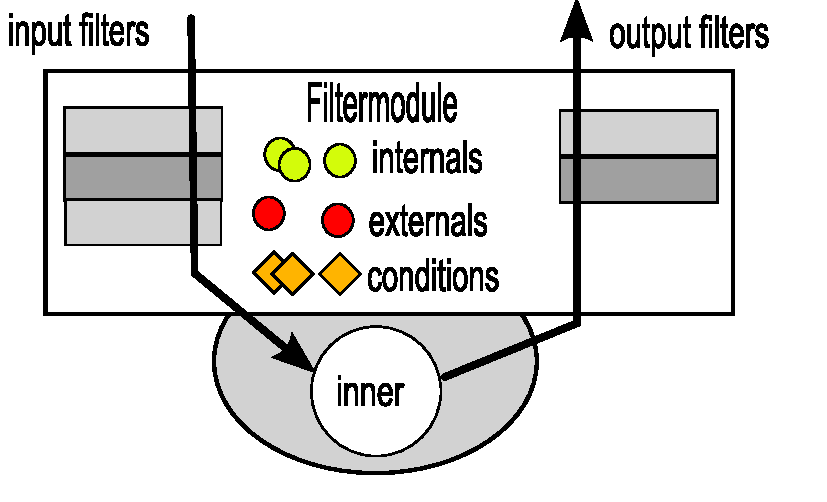
\includegraphics[style= fourthheight]{images/ARM-filtermodule}
	\caption{Schematic representation of a filter module}
	\label{fig::arm::fm:schema}
\end{figure}
A filter module is an entity that holds filter sets which are composed together.
The objects and the conditions that are used in the filters are also declared in the filter module.
\autoref{fig::arm::fm:schema} demonstrates
how a filter module can be visualized in a schema.
The schema shows a filter module superimposed to an object, this object is called the ``inner'' object.
Any message that is sent to the object goes through the input filters and any message that is sent
goes through the output filters. Both filter sets can use internals, externals, and conditions.
These elements are declared in the internals, externals, and conditions blocks.

\section*{Examples}
\begin{lstlisting}[caption={Dynamic strategy filter module from Pacman },label=lst::ARM:fil:example1,style=listing,language=ComposeStar,float=[tpb]]
filtermodule dynamicstrategy{
  internals
    stalk_strategy : pacman.Strategies.StalkerStrategy;
    flee_strategy : pacman.Strategies.FleeStrategy;   
  conditions
    pacmanIsEvil : pacman.Pacman.isEvil();
  inputfilters
    stalker_filter : Dispatch = {!pacmanIsEvil => 
      [*.getNextMove] stalk_strategy.getNextMove};
    flee_filter : Dispatch = {[*.getNextMove] flee_strategy.getNextMove}
}
\end{lstlisting}
\begin{lstlisting}[caption={Enqueue filter module from Jukebox },label=lst::ARM:fil:example2,style=listing,language=ComposeStar,float=[tpb]]
filtermodule Enqueue{
  externals
    playlist: Jukebox.Playlist = Jukebox.Playlist.instance();
  inputfilters
    meta : Meta = { True => [*.play] playlist.enqueue}
}
\end{lstlisting}
A filter module can consist of parameters, internals, externals, conditions, input filters, and output filters.
The blocks in which these filter elements are declared are all optional, so the shortest filter module you can write is \lstinline!filtermodule fm {}!. \autoref{lst::ARM:fil:example1}
and \autoref{lst::ARM:fil:example2} show two example filter modules taken from the \Compose* example directory~\cite{Composestar}. What the separate filter module elements do can be found in their respective
chapters, the examples are given to get an idea of how to build up a filter module.
The ordering of the blocks is fixed, so for instance, it is not possible to place the conditions block before the internals block.

\section*{Legality Rules}
\begin{itemize}[noitemsep]
\item The identifier of a filter module must be unique for the concern where it is declared in;
\item The blocks in a filter module must be in the following ordering: internals, externals, conditions, input filters, and output filters;
\item You can only have one declaration of the above mentioned blocks, for example there can be only one set of internals.
\end{itemize}

%\faq{} no questions, should be clear, I'm not going to think any questions and hints
\comments{
\para{Language Independence}
\begin{lstlisting}[caption = {A filter module with a primitive value}, label = lst::ARM:int:example3,
style = listing, language =ComposeStar, float = tpb]
filtermodule rollbackcounter{
  internals
    counter : int;
  inputfilters
    e : Error = {(if counter > 10) => [*.*]};
    m : Meta = {[*.rollback] counter++;}
}  
\end{lstlisting}
\begin{lstlisting}[caption = {A filter module with an object instead of primitive value}, label = lst::ARM:int:example4,
style = listing, language =ComposeStar, float = tpb]
filtermodule rollbackcounter{
  internals
    counter : Counter; // extends of Integer
  conditions
    greaterThenTen : counter.isGreaterThenTen();
  inputfilters
    e : Error = {greaterThenTen => [*.*]};
    m : Append = {[*.rollback] counter.raiseCounter}
}
\end{lstlisting}
It is not possible to use primitive values, like int, char, and bool, as internals and externals,
this is a result from the language independence
we want to have in \Compose*. 
This means that only objects can be used as internals and externals.
Object references are language independent and thus usable in
a language independent environment.
The usage of primitive values in the language
would break language independence because the primitives have different ranges in each 
language\footnote{For bool (or boolean) this is not a real problem, because generally it has only
two values: True and False. However, if we would find (or create) a language that uses fuzzy
values for its booleans then we have the same range problem with booleans as with, for example, integers.
In such scenario the question is whether the fuzzy range is from one to zero or from hundred to zero?}.
There are ideas to introduce a set of primitive values for usage in the filter module,
but these ideas always get stuck on the fact that you need to set a range for the primitives
and they often conflict with the requirement to keep the language as concise as possible.
An example of a rejected solution is the subtyping of integer values like in the programming language Ada~\cite{Ada95}. With Ada it is possible to create a subtype of integer by declaring
it as a subtype of integer and by setting a range, for instance from one to ten.
A possible Ada type declaration is \lstinline|type OwnInteger is Integer range 0 .. 256;|

If we look on how we would put a primitive into action
we can see that we can do the same with an object. For example, if we take a filter module that allows
ten times the call \lstinline!rollback! and gives an error the eleventh time, then the filter module
does need a counter to keep track on how many times the call \lstinline!rollback! has been send to that
filter module. In \autoref{lst::ARM:int:example3} the code with a primitive value is worked out.
In line 3 of \autoref{lst::ARM:int:example3} an integer is declared, we assume that by default the value will be zero. An alternative is to create an internals declaration like
\lstinline!counter : int = 0;!. This value counter is used in line 5 to check whether the amount of rollback is still
below ten. To get the filter module count every call to the method \lstinline!rollback! we need
a statement as \lstinline!counter++! (Line 6). Because the internal is only accessible in the filter module we need
to use a statement in the filter that raises the value of counter.
So with the use of primitive values in the filter module we also need to add operators to use the values.

\autoref{lst::ARM:int:example4} shows the same behavior only with an object that inherits from the
Integer object\footnote{Extending from Integer makes that you can add your own custom methods like \emph{raise()} and
\emph{isGreaterThenTen()}.}.
The internal declaration now uses a Counter class type, the if-statement is replaced with a condition declaration as seen in line 5 and the raising of the counter is now been handled with a function of the class Counter.
This gives that using an object is preferable to a primitive value, because we can use the
methods of the internal and we do not need to introduce mathematical operators, like
``$>$'' and ``$+$'', in the filter syntax. So we can achieve the same with an object or a primitive,
only with the primitive we have problems with breaking language independence and
we have a syntax that is less concise.

Therefore we conclude that we do not need primitive values in the language and we only need method calls
and object references.
Not adding primitive values to the syntax saves us
from the issues mentioned above. First it offers us the possibility to keep the filter module as concise as possible and
second if we would consider adding primitive values and some operators, we would never become as expressive
as the base language, and it is not our goal to copy all the possibilities of the base language.
With this we can close the discussion whether to introduce primitive values in
the filter module.

\para{The Methods Block}
Originally, the filter module also had a method block. As mentioned earlier in ~\cite{Doornenbal2006} it has become obsolete
and it has been removed from the language.

\para{Combining Internals and Externals}
\begin{lstlisting}[caption = {A parameter as external object}, label = lst::ARM:fm:comment1,
style = listing, language =Composestar, float = tpb]
filtermodule agenda(?externalObject){
  externals
    secretary : Example.Secretary = ?externalObject;
}

superimposition{
  filtermodules
    selA <- example(Example.Secretary);
    selB <- example(Example.Secretary);
}
\end{lstlisting}
The internals and externals are the local variables of a filter module. If we look at the example programs in \Compose*, then we see
that the externals are only used in combination with the singleton design pattern~\cite{Gamma95}. Because
the usage of the externals is limited, we can consider combining both blocks into one block called \emph{variables}.
Whether the combination of both blocks is desirable depends whether we want to keep a visible difference
between an internal and external declaration. A solution is to mark externals with a ``*'', like C++ uses for pointers, so that all the
variables are in one field and there is still a (visible) difference between internals and externals.

However, with the introduction of filter module parameters, the usages of the internals and externals fields are extended.
For the externals it means that we can get programs like \autoref{lst::ARM:fm:comment1}. In that example
one instance of the given object is used for all the classes that are bound in the filter module binding, thus
in this particular example there are two instances of the class \lstinline!Example.Secretary!, one for the selection
of classes of selA and of the classes of selB\footnote{The selections can have an overlap.}.
The external declaration on line 3 has an identifier, a fixed type, and a flexible object.
We can apply the ``*'' construction also in this situation, but then you can only derive the meaning of the code with the ``*''. If we would introduce constructor calls for internal declaration we get a readability problem.
Consider the line of code: \lstinline|variable : type = ?parameter;|. If this would be an internal in the
variable block it means that the parameter is cloned, an external in the same variable field is then
\lstinline|*variable : type = ?parameter;|, which means the same as the construct in \autoref{lst::ARM:fm:comment1}.
Due to the new options introduced by the parameters, keeping the distinction between internals and externals becomes
more preferable over the combination of the two blocks.

So with the introduction of parameters, we need to reevaluate the idea of combining the internals and externals fields.
And can conclude that with the
choice of adding parameters to the filter module, it is better to make a clear distinction between externals and internals,
and the best way to do so is to keep them separated.

\para{Block Ordering}
The order of the blocks in the filter module is fixed, making it impossible, for instance, to place externals before internals and to have two conditions blocks. It is
a matter of readability whether mixed ordering and multiple occurrences of blocks are better then fixed ordering and single occurrence of blocks.
Because of the filter operators and how filters work together we only allow one input and output filter set per filter module and that we do not break it up in sub parts. If we would
break up the filter sets, then it becomes harder to read how a filter set behaves.
Another point is that if we would allow the declaration of internals and externals between filters, then users can get confused whether the scope is the whole filter module or just until the next internals or externals block.
Therefore we chose to use the fixed one-of-a-type syntax and that no mixes of blocks are allowed.
}
%\dotnetcomment{
}
%\javacomment{}
%\ccomment{}
%\pending{}
%\furtherreading{}